\section{Introduction}\label{sec:intro}

Wireless capsule endoscopy (WCE) lets a swallowable camera image the entire
gastrointestinal (GI) tract without sedation, but a finding---a bleed, an
ulcer, a polyp---is only clinically actionable if the clinician knows
\emph{where} along the tract it occurred. Radio-frequency (RF) localization of
the capsule from a small set of body-surface receivers is the leading
non-imaging route to that coordinate. The overwhelming majority of WCE-RF
localization methods, however, report only a \emph{point} estimate of capsule
position. For a quantity a clinician must act on, a point estimate without a
calibrated notion of confidence is incomplete: a \SI{2}{cm} estimate that is
reliably within \SI{2}{cm} and a \SI{2}{cm} estimate that is silently off by
\SI{6}{cm} in the unobservable direction are clinically very different, yet a
point estimator cannot tell them apart.

At a four-receiver budget for the legal Medical Implant Communication Service
(MICS)/MedRadio band \SIrange{401}{406}{MHz}, the scientifically and clinically
valuable contribution is the calibrated posterior: a distribution over capsule
position whose spread is an interpretable, usable measure of uncertainty. We
study the four-receiver MICS/MedRadio budget with the main coherent sub-band at
${\sim}$\SIrange{402}{405}{MHz}~\cite{mics}, and ask whether a generative model
can deliver such a posterior \emph{without} sacrificing point accuracy.

\paragraph*{Scope (declared up front)}
\textbf{All results in this paper come from full-wave CST Studio Suite (CST) simulation};
no measured-phantom or in-vivo data are used. Simulation-first evaluation is
standard practice in this subfield: comparable studies report on simulation or
simulation-dominant evidence~\cite{yoshitake2022,wisanmongkol2024,ye2014,nadimi2014,pourhomayoun2014,hiyoshi2019}.
We use full-wave CST simulation (not a parametric path-loss model), evaluate
under a protocol \emph{stricter} than the random point-wise splits these
comparators use, and identify a physical-phantom companion as the explicit next
evidence gate (Section~\ref{sec:discussion}).
Figure~\ref{fig:study-overview} summarizes this scope and shows that the
evidence chain targets calibrated posterior reporting, not a point-accuracy
leaderboard.

\begin{figure*}[t]
\centering
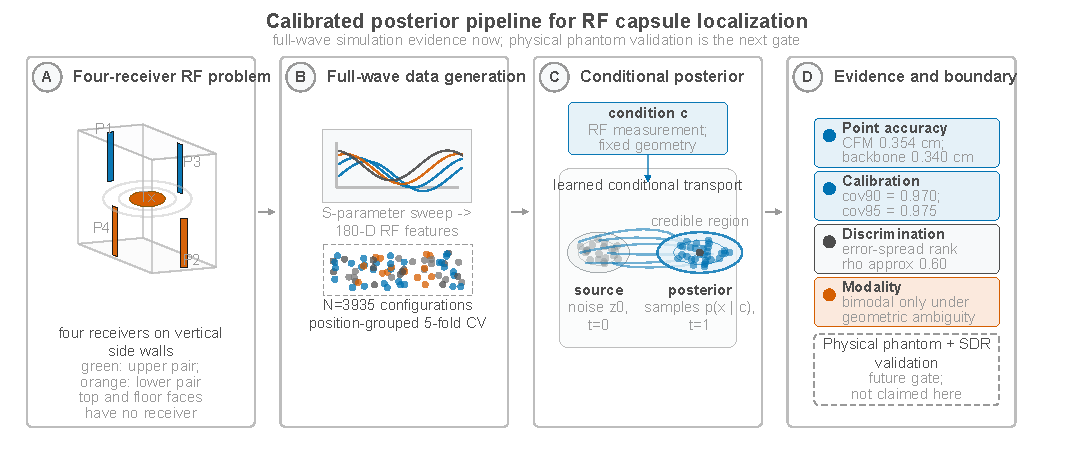
\includegraphics[width=\linewidth]{figures/fig_study_overview.pdf}
\caption{Study overview. A four-receiver MICS/MedRadio budget WCE localization
problem is evaluated with full-wave CST simulation, converted to rich RF
features under position-grouped cross-validation, and solved with a conditional
flow-matching posterior. The figure supports the paper's main claim: the
contribution is the calibrated posterior, with multi-level coverage and
error--spread discrimination while point accuracy remains within \SI{0.014}{cm}
of the backbone (\SI{0.354}{cm} vs \SI{0.340}{cm}). \textbf{Simulation only:}
the physical phantom setup is the next validation gate, not a result claimed in
this paper.}
\label{fig:study-overview}
\end{figure*}

\paragraph*{Contributions and scope}
\textbf{(A) What we do not claim.} We are not the most accurate point estimator at
the four-receiver MICS/MedRadio budget. Real-phantom received signal strength
indicator (RSSI) systems at \SI{2.45}{GHz} report better point
accuracy~\cite{hasnain2026,hasnain2024}, our results are simulation at a ${\sim}6\times$
lower frequency, and our protocol is stricter; we do not contest the
point-accuracy leaderboard. \textbf{(B) What we do claim: the contribution is
the calibrated posterior.}
To our knowledge, this is the first flow-matching/generative WCE-RF position
posterior with empirical multi-level coverage under position-grouped
cross-validation. Concretely:
\begin{enumerate}
\item A clean conditional flow-matching (CFM) posterior that is calibrated
\emph{from its own samples}: near-nominal multi-level coverage
($0.766/0.935/0.944$ on the initial-stage subset; $0.832/0.970/0.975$ in
combined-set CFM-only scoring) and real error--spread discrimination (Spearman
$\rho\approx0.60$).
\item Point accuracy within \SI{0.014}{cm} of the deterministic backbone
(\SI{0.354}{cm} vs \SI{0.340}{cm} 3D MAE) while significantly beating ten
classical regressors on identical position-grouped folds (position-paired
bootstrap, Section~\ref{sec:results}/Table~\ref{tab:point}).
\item The empirical observation that posterior \emph{modality} tracks
forward-operator invertibility in a controlled receiver-array ablation: the CFM
posterior is bimodal when a mirror-symmetric array leaves $y$ unobservable by
construction, and unimodal on the main anti-symmetric side-wall array where the receiver
placement breaks that symmetry.
\item Evidence that the same posterior width carries the aleatoric uncertainty of
an \emph{unknown} capsule orientation, reframing orientation as a nuisance the
posterior integrates over rather than a quantity to be regressed.
\item A feature-deployability ablation on the initial-stage subset ($N=1980$)
that separates
the single-tone, magnitude-only floor (${\sim}\SI{1.5}{cm}$) from the
phase-coherent sub-centimetre regime; these ablation values are therefore not
the combined-set $N=3935$ headline numbers.
\end{enumerate}
The one Bayesian WCE-RF precedent~\cite{nadimi2014} reports RMSE against the
Cram\'er--Rao lower bound on a parametric path-loss simulation with no empirical
coverage, which is why we frame the novelty around the learned posterior and its
empirical coverage rather than around Bayesian localization in general.
Section~\ref{sec:related} surveys WCE-RF localization and the calibrated-posterior
gap; Section~\ref{sec:dataset} describes the simulation and feature pipeline;
Section~\ref{sec:method} defines the CFM posterior; Section~\ref{sec:results}
reports point accuracy, coverage, modality, deployability, and orientation
uncertainty; and Section~\ref{sec:discussion} and Section~\ref{sec:conclusion}
state the scope and physical-phantom gate.
